\documentclass{article}

\usepackage[polish]{babel}
\usepackage[utf8]{inputenc}
\usepackage[T1]{fontenc}
\usepackage{enumitem}
\usepackage[onelanguage]{algorithm2e}
\SetKwInput{KwData}{Dane}
\SetKwInput{KwResult}{Wynik}
\SetKwRepeat{Do}{do}{while}
\usepackage{amsmath}
\usepackage{amssymb}
\usepackage{booktabs}
\usepackage{graphicx}
\usepackage{geometry}
\usepackage{multicol}
\geometry{
a4paper,
total={170mm,257mm},
left=15mm,
right=15mm,
top=30mm,
bottom=30mm
}
\title{Obliczenia Naukowe\\Lista 5\\Laboratoria}
\date{02 stycznia 2017}
\author{Piotr Szyma}


\begin{document}
    \pagenumbering{gobble}
    \maketitle
    \newpage
    \pagenumbering{arabic}
    \section{Zadanie 1}
\subsection{Opis problemu}
Napisać funkcję obliczającą ilorazy różnicowe zgodnie ze specyfikacją podaną w treści zadania bez użycia tablicy dwuwymiarowej (macierzy). \\ $ \texttt{function ilorazyRoznicowe (x::Vector{Float64}, f::Vector{Float64})} $ \\
\subsection{Analiza}
\subsection{Implementacja}
Moja implementacja algorytmu w języku Julia znajduje się w module $ \texttt{MyModule} $ znajdującym się w pliku załączonym do tego sprawozdania. 
    \newpage    
    
\section{Zadanie 2}
\subsection{Opis problemu}
Narysować wykres funkcji $ f(x) = e^x \ln (1 + e^{-x}) $ w co najmniej dwóch dowolnych programach do wizualizacji. Następnie policzyć granicę funkcji $ \lim_{x \to \infty} f(x) $. Porównać
wykres funkcji z policzoną granicą. Wyjaśnić zjawisko.
\subsection{Rozwiązanie}
Oto granica funkcji $ f(x) $:
$$ \lim_{x \to \infty} e^x \ln (1 + e^{-x}) = 1$$
\subsection{Wynik}
Wykresy wygenerowane za pomocą dwóch programów do wizualzacji załączone są na Rysunkach 1 i 2. Kody źródłowe programów dołączyłem do sprawozdania w osobnych plikach. \\\\
Jak widać na wykresach, w pewnym momencie funkcja zaczyna przyjmować nieoczekiwane - błędne - wartości. Głównym czynnikiem wpływającym na takie zachowanie jest operacja mnożenia bardzo dużej liczby $ e^x $ przez bardzo małą liczbę $ \ln(1 + e ^{-x}) $, bo $ \lim_{x \to \infty} \ln (1 + e^{-x}) = 0$.
\begin{figure}[!htbp]
  \centering  
  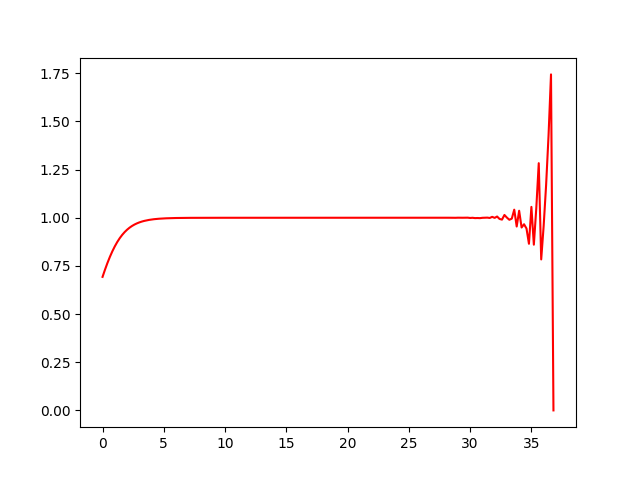
\includegraphics[totalheight=7cm]{../source/task-2/matplotlib.png}
  \caption{Wykres wygenerowany za pomocą biblioteki matplotlib w języku Python}
  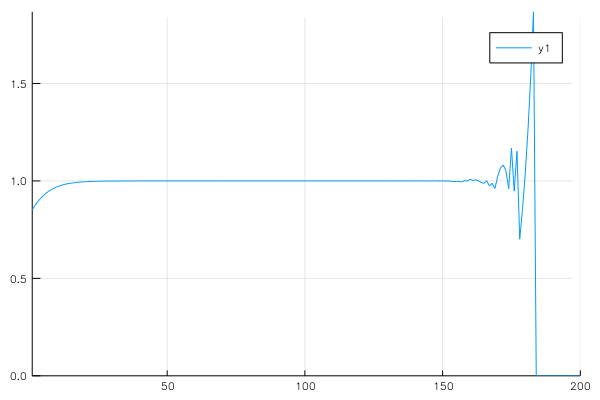
\includegraphics[totalheight=6cm]{../source/task-2/juliaplot.png}
  \caption{Wykres wygenerowany za pomocą biblioteki Plot w języku Julia}
\end{figure}

    \newpage
    \section{Zadanie 3}
\subsection{Opis problemu}
Zadanie polegało na zaimplementowaniu algorytmu rozwiązującego równanie $ f(x) = 0 $ $\textsc{metodą siecznych} $.
\subsection{Pseudokod}
\begin{algorithm}[H]
  \KwData{$f, a, b, M, \delta, \epsilon$}
  \KwResult{$x, f(x), i, err$}
  $f_a \leftarrow f(a);$ $f_b \leftarrow f(b)$\\
  \Do{$ k < M $}{
    $ k \leftarrow k + 1 $ \\
    \If{$ |f_a| > |f_b| $}{
      $a \leftrightarrow b$; $f(a) \leftrightarrow f(b)$ 
    }
    $ s \leftarrow \frac{b - a}{f_b - f_a}$ \\
    $ b \leftarrow a$; $ f_b \leftarrow f_a$  \\ 
    $ a \leftarrow a - f_a * s $  \\ 

    \If{$ |b - a| < \delta \lor |f_a| < \epsilon $}{
      return $ (a, f_a, k, 0) $;
    }
  }
  return $ (a, f_a, M, 1) $;  
\end{algorithm}
\subsection{Implementacja}
Moja implementacja algorytmu w języku Julia znajduje się w module $ \texttt{MyModule} $ znajdującym się w pliku załączonym do tego sprawozdania.
\end{document}